\chapter{表面重建} \label{chap3}
\section{引言}
为了计算表面张力,我们需要一种能够从点云中获取表面和表面法向的方法。本文使用的方法是
使用粒子水平集方法[**]获得一个粗糙的一阶连续隐式曲面,并使用MarchingCube[**]算法重构表面网格。然而该网格
的质量只能做到一阶连续,计算得到的法向在面片之间并不连续,难以应用在表面张力所需的法向计算。本文在该网格
上进行泊松圆盘采样,然后结合已经存在的IPIA算法,提出一种新的快速重建算法以此获得一个二阶光滑
的隐式曲面,然后基于该隐式曲面来计算表面点云的法向。
\section{粒子水平集方法}
记$\mathcal{V}$为点云集合,$v\in \mathcal{V}$为粒子,记$d(x,v)\in \mathbb{R}$为空间上$x$的点到粒子$v$的距离,
则$\mathcal{S}(v) = \{x\in \mathbb{R}^3: d(x,v) = r\}$为半径为$r$,圆心在$v$的球,如图\ref{fig:particle levelset}左所示,蓝色圆圈为二位情况的$\mathcal{S}(v)$。
\begin{figure}[htbp]
    \centering
    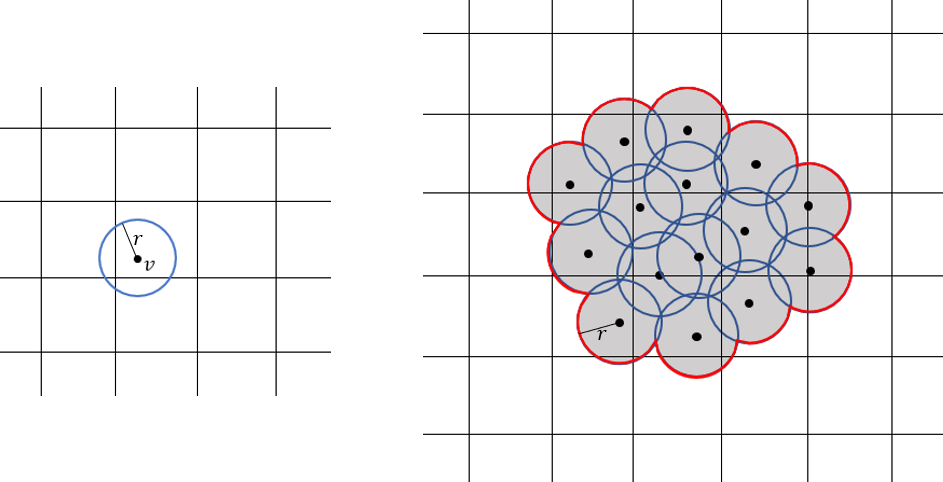
\includegraphics[scale=1.0]{./images/image3.png}
    \caption{二维情况$\mathcal{S}(v)$(左)与$\mathcal{S}(\mathcal{V})$(右)}
    \label{fig:particle levelset}
\end{figure}

记$d(x,\mathcal{V}):= \min \{ d(x,v): v\in \mathcal{V}\}$,则$\mathcal{S}(\mathcal{V}) = \{x\in \mathbb{R}^3: d(x,\mathcal{V}) = r\}$为点云的球外延边界。

如图\ref{fig:particle levelset}右所示,红色的外延边界为所求$\mathcal{S}(\mathcal{V})$。该红色边界初步确定了该点云的边界,灰色部分界定了物体内部。下一步我们将从利用红色边界和背景网格提取出
一个粗糙的网格。

\section{水平集网格提取}
Marching cube通常用于三维标量场的水平集的可视化,本文使用Marching cube算法来获取水平集的三角网格,在本文中我们的水平集为
$\mathcal{S}(\mathcal{V}) = \{x\in \mathbb{R}^3: d(x,\mathcal{V}) = r\}$。


\begin{figure}[htbp]
    \centering
    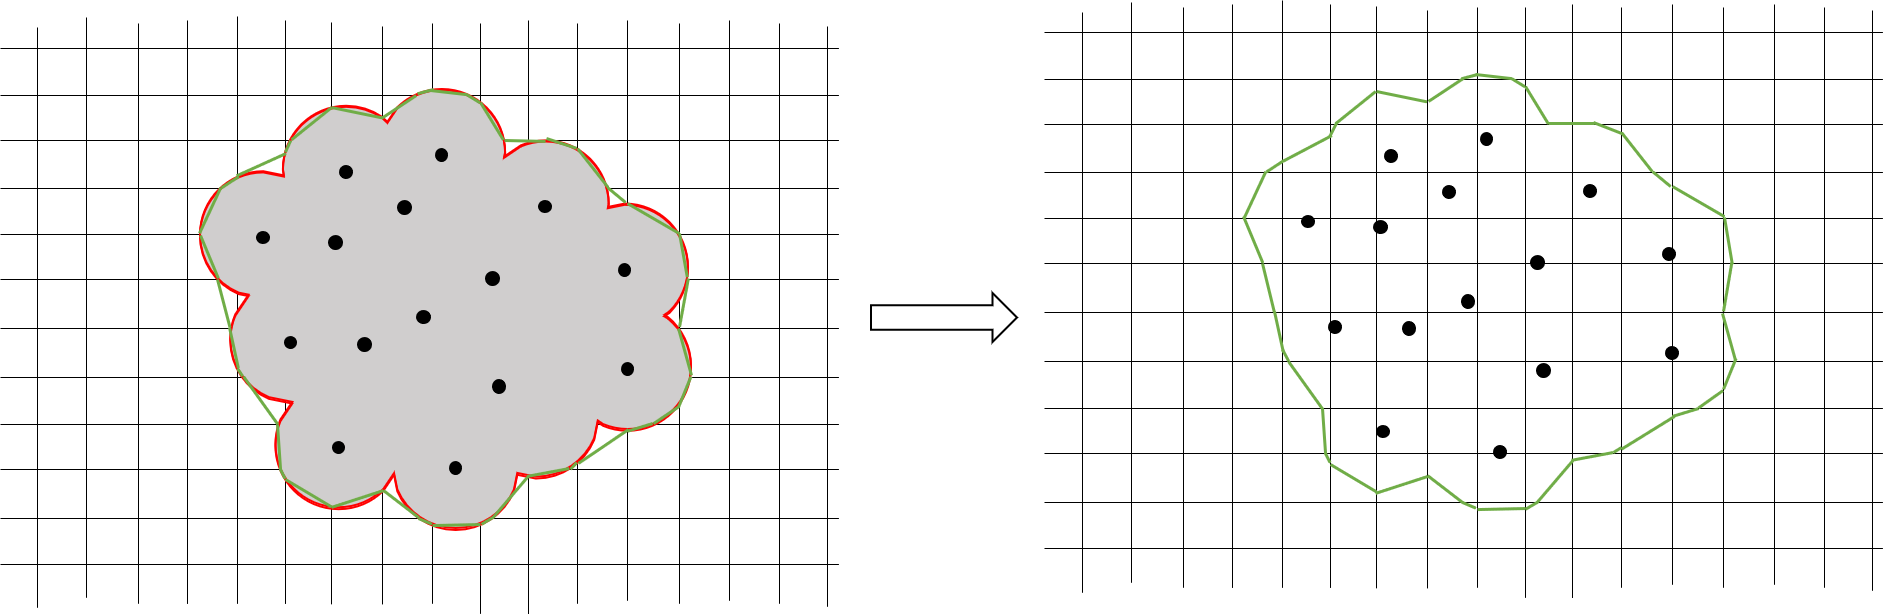
\includegraphics[scale=0.3]{./images/image7.png}
    \caption{二维点云轮廓提取图示}
    \label{fig:2D marching cube}
\end{figure}
\begin{figure}[htbp]
    \centering
    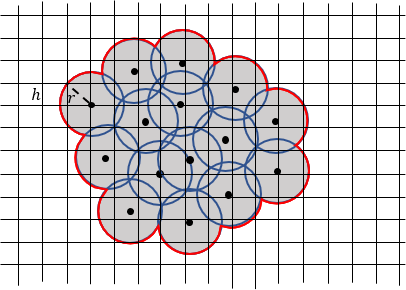
\includegraphics[scale=1.0]{./images/image5.png}
    \caption{二维情况的$r$与$h$的关系}
    \label{fig:grid and sphere}
\end{figure}

本小节我们的目标只是提取出一个大致的点云的表面轮廓,如图\ref{fig:2D marching cube}所示。我们首先将空间离散化成一个个均匀的立方体,我们称之为背景网格,并对每一个正方体格点放置一个标志符,默认为0,此处记立方体宽度为$h$,为了保证球能够覆盖到一个足够大的
面积,此处我们选择$r = \sqrt{3}h$,二维情况为$r = \sqrt{2}h$,具体如图\ref{fig:grid and sphere}所示。本文为了节省内存,
具体实现使用了八叉树数据结构。之后对每一个粒子操作,将粒子周围的格点做标记,如果格点距离该粒子半径不超过
$r$,则将格点标记为1,如此下来,所有的正方体格点都被标记为两种状态。之后我们对正方体按格点状态进行分类,由于每个格点有
两种状态,每个正方体有8个格点,如此一来便有$2^8 = 256$种状态,在合并旋转和对称的情况后,可以简化成15种,可以分类成如图\ref{fig:marching cube table}所示。
\begin{figure}[htbp]
    \centering
    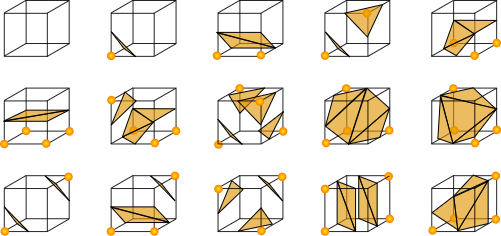
\includegraphics[scale=0.6]{./images/image6.png}
    \caption{Marching cube列表}
    \label{fig:marching cube table}
\end{figure}
之后我们再将网格顶点位置调整到合适的位置,并建立三角网格数据结构。具体的算法描述见\textbf{Algorithm \ref{alg:marching cube}}。
\begin{algorithm}
    \caption{Marching cube}
    \label{alg:marching cube}
    \begin{algorithmic}[1]
    \Require 点云集合$\mathcal{V}$,立方体宽度$h$
    \Ensure 三角网格位置集合$V$,面片集合$F$
    \State 准备空间网格数据结构(八叉树),并记$\mathcal{G}$为格点集合,$\mathcal{E}$为立方体的边集合,$\mathcal{C}$为立方体集合
    \State $state(g)\in \{0,1\}$为格点$g\in \mathcal{G}$的状态,初始化为0
    \State $P(e)\in \mathbb{R}^3$为边$e\in \mathcal{E}$上的一个顶点
    \State $r = \sqrt{3}h$
    \For{$v\in \mathcal{V}$}
        \For{$g \in \{g\in \mathcal{G}: \Vert g - v\Vert < r\}$}
            \State $state(g)$标记为1    
        \EndFor
    \EndFor    
    \For{$e \in \{e\in \mathcal{E}: e\text{两端格点状态相异}\}$}
      \State  取$e$状态为$1$的顶点记为$g_1$,状态为$0$的记为$g_0$
      \State 申请栈空间$p_{stack}$
      \For{$v \in \{v\in \mathcal{V}: \Vert g_1 - v\Vert < r\}$}
        \State 计算$\mathcal{S}(v)$与$e$的交点并压入$p_{stack}$中
      \EndFor
      \State 在$p_{stack}$中选取离$g_0$最近的点,并赋值给$P(e)$,同时将$P(e)$压入$V$中
    \EndFor
    \For{$c \in \mathcal{C}$}
        \State 匹配$c$所对应的Marching cube 列表中的状态
        \State 构造相应的三角面表$f_s$,顶点选为对应$P(e)$在$V$中得索引
        \State 将$f_s$其压入$F$中
    \EndFor
    \end{algorithmic}
\end{algorithm}


\textsf{在这里补点三维图,说明网格质量不行,只能一阶连续,法向不连续}


从实验结果的图中可以发现,Marching cube算法确实提取出了一个点云的边界轮廓,但是轮廓只能做到一阶连续,法向明显不连续,同时其三角网格质量无法
无法保证,甚至可以明显看出在一些尖锐地方,网格质量极差,上述的问题给我们计算表面张力带来了很大的阻碍。

\section{LSIPIA}
为了解决法向不连续的问题以及网格质量差的问题,我们使用二阶连续的隐式曲面来逼近三角网格,因此隐式曲面的法向一阶连续。

\subsection{隐式曲面的渐进迭代逼近}
我们首先给出隐式曲面重建问题,给定一个无序点集$\mathcal{V} = \{v_i = (v_i^1,v_i^2,v_i^3)\}_{i = 1}^n$以及点
上的单位法向量$\mathcal{N} = \{n_i = (n_i^1, n_i^2, n_i^3)\}_{i = 1}^n$,寻找一个函数$f(x^1,x^2,x^3)$使得
$f(x^1,x^2,x^3)$的$0$水平集拟合该组无序点集$\mathcal{V}$。以数学的表达形式即为
\begin{equation}
    \begin{split}
        \min_f\sum_{i = 1}^{n} f(v_i^1,v_i^2,v_i^3)^2       
    \end{split}
\end{equation}
为了让问题可解,我们选择$f$为有限个张量积B-样条基函数的线性组合,即$$f(x^1,x^2,x^3) = \sum_{i = 1}^{N_x}\sum_{j = 1}^{N_y}\sum_{k = 1}^{N_z} C_{ijk}B_i(x^1)B_j(x^2)B_k(x^3)$$
这里我们选择二阶B-样条基函数,其中二阶标准B-样条函数
$$B(x) = \begin{cases}
    \frac{3}{4} - \left | x \right | ^2  & 0 \leq \left | x \right | < \frac{1}{2}\\
    \frac{1}{2}(\frac{3}{2} - \left | x \right |)^2 & \frac{1}{2}\leq \left | x \right | <\frac{3}{2}\\
    0 & \frac{3}{2} \leq \left | x \right |
   \end{cases}$$
如图\ref{fig: standard B-spline basis}所示,这里$B_i(x) := B(\frac{1}{h}(x - x_i))$,这里的$x_i$本文选取为空间立方体网格格点坐标的一个分量,$h$为立方体宽度。
\begin{figure}[htbp]
    \centering
    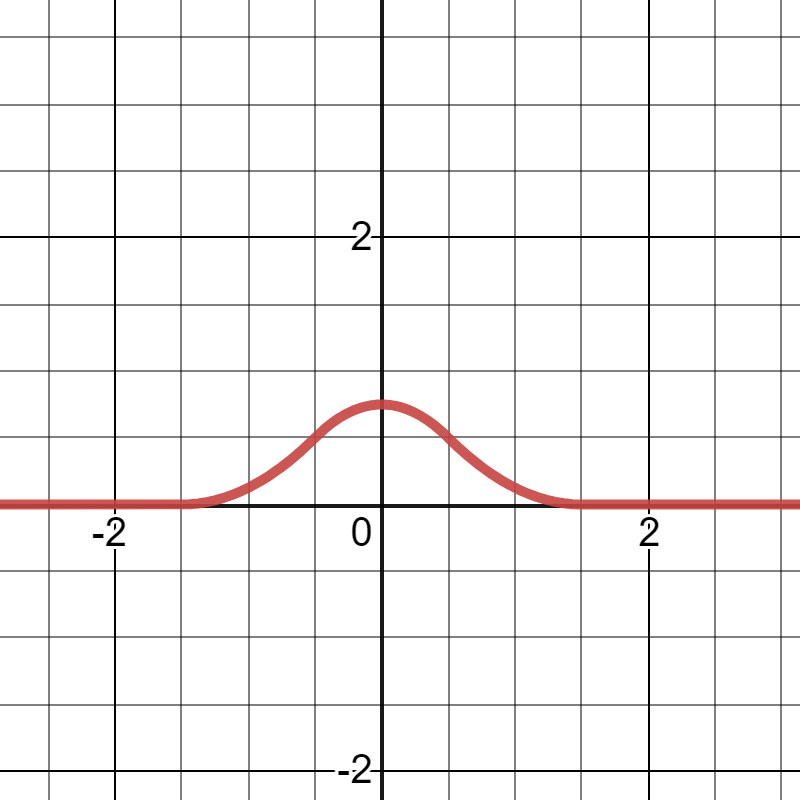
\includegraphics[scale=0.2]{./images/image8.png}
    \caption{二次标准B-样条基函数}
    \label{fig: standard B-spline basis}
\end{figure}
则最小化问题(3.2)转化成
\begin{equation}
    \begin{split}
        \min_{C_{ijk}}E(C_{111},C_{112},...,C_{N_xN_yN_z}):=\frac{1}{2}\sum_{i = 1}^{n} f(v_i^1,v_i^2,v_i^3)^2 
    \end{split}
\end{equation}
这里$C_{ijk}$张量积B-样条系数。

我们记三变量B-样条基函数为$B_{ijk}(x^1,x^2,x^3) = B_i(x^1)B_j(x^2)B_k(x^3)$,则上述问题变为
\begin{equation}
    \begin{split}
        &\min_{C_{ijk}}E(C_{111},C_{112},...,C_{N_xN_yN_z}):= \frac{1}{2}\sum_{r = 1}^{n} (\sum_{ijk}C_{ijk}B_{ijk}(v_r^1,v_r^2,v_r^3))^2 \\
        &\Leftrightarrow \delta E(\{C_{ijk}\}) = 0\\
        &\Leftrightarrow \delta (\frac{1}{2}\sum_{r = 1}^{n} (\sum_{ijk}C_{ijk}B_{ijk}(v_r^1,v_r^2,v_r^3))^2) = 0\\
        &\Leftrightarrow \sum_{r = 1}^{n} \sum_{ijk} \sum_{uvw}C_{ijk}B_{ijk}(v_r^1,v_r^2,v_r^3)B_{uvw}(v_r^1,v_r^2,v_r^3)\delta C_{uvw} = 0\\
        &\Leftrightarrow \sum_{r = 1}^n \sum_{ijk} C_{ijk} B_{ijk}(v_r^1,v_r^2,v_r^3)B_{uvw}(v_r^1,v_r^2,v_r^3) = 0
    \end{split}
\end{equation}
我们将$\{B_{111},B_{112},...,B_{11N_z},...,B_{1Ny1},...B_{N_xN_yN_z}\}$以字典序排列,这样我们可配置如下矩阵
\begin{align*}
    \mathbf{B} = \begin{bmatrix}
        B_{111}(v_1^1,v_1^2,v_1^3) & B_{112}(v_1^1,v_1^2,v_1^3) &...& B_{N_xN_yN_z}(v_1^1,v_1^2,v_1^3)\\
        B_{111}(v_2^1,v_2^2,v_2^3) & B_{112}(v_2^1,v_2^2,v_2^3) &...& B_{N_xN_yN_z}(v_2^1,v_2^2,v_2^3)\\
         \vdots & \vdots & & \vdots\\
        B_{111}(v_r^1,v_r^2,v_r^3) & B_{112}(v_r^1,v_r^2,v_r^3) &...& B_{N_xN_yN_z}(v_r^1,v_r^2,v_r^3)\\
    \end{bmatrix}
\end{align*}
同样对于$\{C_{111},...,C_{N_xN_yN_z}\}$我们有
\begin{align*}
    \mathbf{C} = \begin{bmatrix}
        C_{111} \\
        \vdots \\
        C_{N_xN_yN_z}\\
    \end{bmatrix}
\end{align*}
代入(3.3)最后一个式子中,我们可以得到一个紧凑的形式
$$\mathbf{B}^T \mathbf{B} \mathbf{C} = 0$$
然而,在实践中以上线性系统并非有唯一解,并且有平凡解($\mathbf{C} = 0$)。为了避免陷入平凡解,我们添加法向扰动。
我们利用本小节开头提到的每一点上的法向信息$\mathcal{N}$,我们利用法向取一些偏移点$\mathcal{Q} = \{q_i = v_i + \epsilon n_i: v_i \in \mathcal{V}, n_i \in \mathcal{N}\}$。
然后尽可能要求$f(q_i) = \epsilon, i = 1,2,3,...n$。据此我们修改(3.3)中的优化问题,
\begin{equation}
    \begin{split}
        &\min_{C_{ijk}}E(C_{111},C_{112},...,C_{N_xN_yN_z}):= \frac{1}{2}\sum_{r = 1}^{n} [ (\sum_{ijk}C_{ijk}B_{ijk}(v_r^1,v_r^2,v_r^3))^2 + (\epsilon - \sum_{ijk}C_{ijk}B_{ijk}(q_r^1,q_r^2,q_r^3))^2]\\
        &\Leftrightarrow \sum_{r = 1}^n (\sum_{ijk}C_{ijk} B_{ijk}(v_r^1,v_r^2,v_r^3)B_{uvw}(v_r^1,v_r^2,v_r^3) - ( \epsilon - \sum_{ijk} C_{ijk}B_{ijk}(q_r^1,q_r^2,q_r^3) )B_{uvw}(q_r^1,q_r^2,q_r^3))\\
    \end{split}
\end{equation}

\begin{align*}
    \mathbf{B} = \begin{bmatrix}
        B_{111}(v_1^1,v_1^2,v_1^3) & B_{112}(v_1^1,v_1^2,v_1^3) &...& B_{N_xN_yN_z}(v_1^1,v_1^2,v_1^3)\\
        B_{111}(v_2^1,v_2^2,v_2^3) & B_{112}(v_2^1,v_2^2,v_2^3) &...& B_{N_xN_yN_z}(v_2^1,v_2^2,v_2^3)\\
         \vdots & \vdots & & \vdots\\
        B_{111}(v_r^1,v_r^2,v_r^3) & B_{112}(v_r^1,v_r^2,v_r^3) &...& B_{N_xN_yN_z}(v_r^1,v_r^2,v_r^3)\\
        B_{111}(q_1^1,q_1^2,q_1^3) & B_{112}(q_1^1,q_1^2,q_1^3) &...& B_{N_xN_yN_z}(q_1^1,q_1^2,q_1^3)\\
        B_{111}(q_2^1,q_2^2,q_2^3) & B_{112}(q_2^1,q_2^2,q_2^3) &...& B_{N_xN_yN_z}(q_2^1,q_2^2,q_2^3)\\
        \vdots & \vdots & & \vdots\\
        B_{111}(q_r^1,q_r^2,q_r^3) & B_{112}(q_r^1,q_r^2,q_r^3) &...& B_{N_xN_yN_z}(q_r^1,q_r^2,q_r^3)\\
    \end{bmatrix}
\end{align*}
如果再记
\begin{align*}
    \mathbf{b} = \begin{bmatrix}
        0\\
        \vdots\\
        0\\
        \epsilon \\
        \vdots \\
        \epsilon
    \end{bmatrix}
\end{align*}
其中$\mathbf{b}$的前$n$项为$0$,后$n$项为$\epsilon$。则(3.4)式可以写成紧凑的形式
\begin{equation}
    \mathbf{B}^T ( \mathbf{b} - \mathbf{B} \mathbf{C}) = 0    
\end{equation}
求解该线性系统,我们使用迭代法求解,与IPIA[**]不同,我们的迭代格式为
\begin{equation}
\mathbf{C}^{\alpha + 1} = \mathbf{C}^{\alpha} + \Lambda \mathbf{B}^T(\mathbf{b} - \mathbf{B}\mathbf{C}^{\alpha}) , \alpha = 0,1,2...
\end{equation}
这里$\Lambda$为
\begin{equation}
    \begin{split}
        \begin{bmatrix}
            \frac{1}{\sum_{r = 1}^n B_{111}(v_r) +B_{111}(q_r)} & 0 & ... & 0\\
            0 & \frac{1}{\sum_{r = 1}^n B_{112}(v_r) +B_{112}(q_r)} & ... & 0\\
            \vdots & \vdots & ... & \vdots \\
            0 & 0 & ... & \frac{1}{\sum_{r = 1}^n B_{N_xN_yN_z}(v_r) +B_{N_xN_yN_z}(q_r)} \\
        \end{bmatrix}
    \end{split}
\end{equation}
这里$B_{ijk}(x) = B_{ijk}(x^1,x^2,x^3)$,并假设$\Lambda$可逆(即$\forall ijk ,\sum_{r = 1}^n B_{ijk}(v_r) +B_{ijk}(q_r) \neq 0$),否则认为有某个节点$ijk$满足$\sum_{r = 1}^n B_{ijk}(v_r) +B_{ijk}(q_r) = 0$,由于B-样条基函数非负,则$B_{ijk}(v_r) = B_{ijk}(q_r) = 0$,我们可以去掉该节点,同时去掉对应的$\mathbf{B}$和$\mathbf{C}$对应的行,其并不影响点云附近的隐式曲面构建。
所以我们不妨假定$\Lambda$可逆。有关收敛性的证明,详见[**]。本迭代格式相较于IPIA格式最大的优势就是内存占用少,可高度并行,我们从\textbf{Algorithm \ref{alg:LSIPIA}}来分析这一点。

我们可以发现\textbf{Algorithm \ref{alg:LSIPIA}}在第4行,第15行,第22行对应的循环可高度并行。同时需要的额外内存为储存在每个格点$\mathcal{G}$上的$C_{ijk}$,$\lambda_{ijk}$,$\Delta_{ijk}$。而这一点,我们将在下一节中
说明里所需的额外内存可以借用物质点法中的数据结构完成,也就是说LSIPIA的优势为可复用物质点法的数据结构,同时可以高度并行。

[***************************补充实验数据说明速度快****************************]
\begin{algorithm}
    \caption{LSIPIA}
    \label{alg:LSIPIA}
    \begin{algorithmic}[1]
    \Require 点云位置$\mathcal{V}$,点云法向$\mathcal{N}$,背景网格格点集合$\mathcal{G}$,指定迭代次数$LoopTimes$
    \Ensure 隐式曲面$f(x) = \sum_{ijk} C_{ijk}B_{ijk}(x)$,即输出参数值$C_{ijk}$
    \State 初始化$\forall ijk,C_{ijk} = 0$
    \State 初始化$\forall ijk,\lambda_{ijk} = 0$
    \State 初始化偏移量$\epsilon$
    \For{$r \in \#\mathcal{V}$}
        \State 预计算下标为$I = \{ijk : v_r \in supp(B_{ijk})\}$的张量积B-样条函数,储存为$B_{ijk}(v_r)$
        \For{$ijk \in I$}
            \State $\lambda_{ijk} \leftarrow \lambda_{ijk} + B_{ijk}(v)$
        \EndFor
        \State $v_{\epsilon r} \leftarrow v_r + \epsilon n_r$
        \State 预计算下标为$I_{\epsilon} = \{ijk : v_{\epsilon r} \in supp(B_{ijk})\}$的张量积B-样条函数,储存为$B_{ijk}(v_{\epsilon r})$
        \For{$ijk \in I_{\epsilon}$}
            \State $\lambda_{ijk} \leftarrow \lambda_{ijk} + B_{ijk}(v_{\epsilon r})$
        \EndFor
    \EndFor
    
    \For{$ijk \in \mathcal{G}$}
        \If {$\lambda_{ijk}\neq 0$} 
            \State $\lambda_{ijk}\leftarrow \frac{1}{\lambda_{ijk}}$
        \EndIf
    \EndFor

    \State 初始化$\forall ijk,\Delta_{ijk} = 0$
    \For{$i = 1,\dots,LoopTimes$}
        \For{$r \in \#\mathcal{V}$}
            \State 预计算下标为$I = \{ijk : v_r \in supp(B_{ijk})\}$的张量积B-样条函数,储存为$B_{ijk}(v_r)$
            \State $res = 0$
            \For{$ijk \in I$}
                \State $res \leftarrow res + B_{ijk}(v_r)$ 
            \EndFor
            \State $\delta_r = 0 - res$
            \For{$ijk \in I$}
                \State $\Delta_{ijk}\leftarrow \Delta_{ijk} + \delta_r \cdot B_{ijk}(v_r)$ 
                \State 重置$\Delta_{ijk}$为0
            \EndFor
        \EndFor
    \EndFor

    \end{algorithmic}
\end{algorithm}

\subsection{快速法向计算}
在完成\textbf{Algorithm \ref{alg:LSIPIA}}之后,我们获得了一个二阶连续的隐式曲面。即
\begin{equation}
    f(x) = \sum_{ijk} C_{ijk}B_{ijk}(x)
\end{equation}
获取法向我们可以直接计算其梯度$\nabla f$,我们首先分析计算一个点上的梯度所需要的代价。
首先根据张量积B-样条函数的定义$B_{ijk}(x) = B_i(x^1) * B_j(x^2) * B_k(x^3)$,如果选取的为二次样条,则在二维情况下
其能够覆盖到点$x$的基函数如图\ref{fig:2D basis},所以能够覆盖到点$x$的坐标个点为$I = \{ij: i = i_0 + k, j = i_0 + l, \text{其中}k, l \in \{0,1,2\}\}$。
\begin{figure}[htbp]
    \centering
    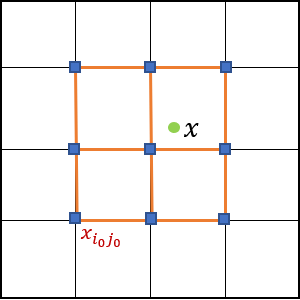
\includegraphics[scale=1.0]{./images/image9.png}
    \caption{蓝色正方形为其紧支集能够覆盖$x$的自由度,$x_{i_0j_0}$为左下角格点坐标}
    \label{fig:2D basis}
\end{figure}

而
\begin{equation}
    \begin{split}
        \nabla f &= \sum_{ijk} C_{ijk} \nabla B_{ijk}(x)\\
        &= \sum_{ijk} C_{ijk} \nabla (B_i(x^1)B_j(x^2)B_k(x^3))\\
        &= \sum_{ijk} C_{ijk} (\partial_i B_i(x^1) \cdot B_j(x^2)B_k(x^3), B_i(x^1)\partial_2 B_j(x^2)\cdot B_k(x^3), B_i(x^1)B_j(x^2)\partial_3B_k(x^3))\\
    \end{split}
\end{equation}
可以发现要计算$x$点的梯度$\nabla f$, 我们需要计算的有$B_i(x^r),\partial_r B_i(x^r), i \in \{0,1,2\}, r \in \{1,2,3\}$,其中样条阶数越高,计算$\partial_r B_i(x^r)$代价越大,并且$\partial_r B_i(x^r)$为分段函数,故在不同的$r$之间不可能做到单指令多数据流并行,同样在拼装
$\nabla B_{ijk}(x)$时每一个维度需要单独的计算。基于这些缺点,我们提出另一个近似法向的计算方法。这里我们使用移动加权最小二乘来逼近格点系数,我们将会看到在
格点张量积B-样条基下,移动加权最小二乘将有惊人的简单形式。

我们寻求的近似目标函数为
\begin{equation}
    f_y (x;c) = f(y) + c^T(x - y)    
\end{equation}

能量函数设计如下
\begin{equation}
    \begin{split}
        E_y(c) = \frac{1}{2} \sum_{ijk} B_{ijk}(y)(f_y(x_{ijk};c) - C_{ijk})^2
    \end{split}
\end{equation}
对上式取极小我们得到
\begin{equation}
    \begin{split}
        0& = \frac{\partial}{\partial c} E_y(c)\\
        &= \frac{\partial}{\partial c} \frac{1}{2}\sum_{ijk} B_{ijk}(y)(f(y) + c^T (x_{ijk} - y) - C_{ijk})^2\\
        &= \sum_{ijk} B_{ijk}(y)(f(y) + c^T (x_{ijk} - y) - C_{ijk}) (x_{ijk} - y)^T\\
        &= \sum_{ijk} B_{ijk}(y)(f(y) - C_{ijk})(x_{ijk} - y)^T + c^T\sum_{ijk}B_{ijk}(y)(x_{ijk} - y)(x_{ijk} - y)^T\\ 
    \end{split}
\end{equation}
则 $$\sum_{ijk} B_{ijk}(y) (C_{ijk} - f(y)) (x_{ijk} - y) = [\sum_{ijk}B_{ijk}(y)(x_{ijk} - y)(x_{ijk} - y)^T]c $$
当然我们要计算$c$我们得到如下式子
\begin{equation}
    c = [\sum_{ijk}B_{ijk}(y)(x_{ijk} - y)(x_{ijk} - y)^T]^{-1} \cdot \sum_{ijk} B_{ijk}(y) (C_{ijk} - f(y)) (x_{ijk} - y)
\end{equation}
这里(3.12)式要成立的条件为$[\sum_{ijk}B_{ijk}(y)(x_{ijk} - y)(x_{ijk} - y)^T]$可逆,我们接下来证明该矩阵可逆。

此处我们记$A = \sum_{ijk}B_{ijk}(y)(x_{ijk} - y)(x_{ijk} - y)^T$。首先我们计算$A$的非对角项即$A_{uv}, u\neq v\text{其中} u,v \in \{1,2,3\}$,这里再记$w \in \{1,2,3\}\text{且} w \notin \{u,v\} $。
即
\begin{equation}
    \begin{split}
        A_{uv} &= \sum_{i_1 i_2 i_3} B_{i_1 i_2 i_3}(y) (x_{i_1 i_2 i_3}^u - y^u)(x_{i_1 i_2 i_3}^v - y^v)\\
        & = \sum_{i_u i_v i_w} B_{i_u}(y^u)B_{i_v}(y^v)B_{i_w}(y^w) (x_{i_u i_v i_w}^u - y^u)(x_{i_u i_v i_w}^v - y^v)\\
        & = \sum_{i_w}B_{i_w}(y^w)(\sum_{i_u}B_{i_u}(y^u)(x_{i_u i_v i_w}^u - y^u))(\sum_{i_v}B_{i_v}(y^v)(x_{i_u i_v i_w}^v - y^v))\\
        & =  \sum_{i_w}B_{i_w}(y^w)(\sum_{i_u}B_{i_u}(y^u)x_{i_u i_v i_w}^u - y^u\sum_{i_u}B_{i_u}(y^u))(\sum_{i_v}B_{i_v}(y^v)x_{i_u i_v i_w}^v - y^v\sum_{i_v}B_{i_v}(y^v))
    \end{split}
\end{equation}

这里我们注意到B-样条基函数的单位分解性$\sum_i B_i(x) = 1$以及线性还原性$\sum_i x_iB_i(x) = x$,带入到
(3.13)式中我们有
$$\sum_{i_w}B_{i_w}(y^w)(\sum_{i_u}B_{i_u}(y^u)x_{i_u i_v i_w}^u - y^u\sum_{i_u}B_{i_u}(y^u))(\sum_{i_v}B_{i_v}(y^v)x_{i_u i_v i_w}^v - y^v\sum_{i_v}B_{i_v}(y^v)) = 0$$
因此$u\neq v\text{时}A_{uv} = 0$,即$A$为对角阵。

接下来考察$u = v$时$A_{uv}$的值,而
\begin{equation}
    \begin{split}
        A_{uu} &= \sum_{i_1 i_2 i_3} B_{i_1 i_2 i_3}(y) (x_{i_1 i_2 i_3}^u - y^u)^2\\
            &= \sum_{i_u i_v i_w} B_{i_u}(y^u)B_{i_v}(y^v)B_{i_w}(y^w)(x_{i_1 i_2 i_3}^u - y^u)^2\\
            &= \sum_{i_u} B_{i_u}(y^u) (x_{i_1 i_2 i_3}^u - y^u)^2 \sum_{i_v}B_{i_v}(y^v)\sum_{i_v}B_{i_w}(y^w)\\
            &= \sum_{i_u} B_{i_u}(y^u) (x_{i_1 i_2 i_3}^u - y^u)^2\\ 
    \end{split}
\end{equation}
我们将说明$\sum_{i_u} B_{i_u}(y^u)(x_{i_1i_2i_3}^u - y^u)$恒为常数。这里我们注意到均匀n阶B-样条导数公式为$\frac{d}{dy} B_i^n(y) = B_i^{n-1}(y+\frac{1}{2}) - B_i^{n-1}(y - \frac{1}{2})$,
此处假定样条阶数为$n$,同时再记$B_{i_u}(y^u)$为$B_{i_u}^n(y^u)$,现在考察$\sum_{i_u} B_{i_u}(y^u)(x_{i_1i_2i_3}^u - y^u)$导数
\begin{equation}
    \begin{split}
        &\frac{d}{dy^u}\sum_{i_u} B_{i_u}^n(y^u) (x_{i_1 i_2 i_3}^u - y^u)^2\\ 
        &= \sum_{i_u} \frac{d}{dy^u} B_{i_u}^n(y^u) (x_{i_1 i_2 i_3}^u - y^u)^2\\
        &= \sum_{i_u} [\frac{d}{dy^u} B_{i_u}^n(y^u)] (x_{i_1 i_2 i_3}^u - y^u)^2 + B_{i_u}^n(y^u)\frac{d}{dy^u}[(x_{i_1 i_2 i_3}^u - y^u)^2]\\
        &= \sum_{i_u} [\frac{d}{dy^u} B_{i_u}^n(y^u)] (x_{i_1 i_2 i_3}^u - y^u)^2 + 2B_{i_u}^n(y^u)(y^u - x_{i_1i_2i_3}^u)\\
        &= \sum_{i_u} [\frac{d}{dy^u} B_{i_u}^n(y^u)] (x_{i_1 i_2 i_3}^u - y^u)^2\\
        &= \sum_{i_u} (B_{i_u}^{n-1}(y^u + \frac{h}{2}) - B_{i_u}^{n-1}(y^u - \frac{h}{2})) (x_{i_1 i_2 i_3}^u - y^u)^2\\
        &= \sum_{i_u} B_{i_u}^{n-1}(y^u + \frac{h}{2}) (y^u - x_{i_1 i_2 i_3}^u)^2 - \sum_{i_u}B_{i_u}^{n-1}(y^u - \frac{h}{2}) (y^u - x_{i_1 i_2 i_3}^u)^2\\   
        &= \sum_{i_u} B_{i_u}^{n-1}(y^u + \frac{h}{2}) (y^u + \frac{h}{2} - x_{i_1 i_2 i_3}^u - \frac{h}{2})^2 -  \sum_{i_u} B_{i_u}^{n-1}(y^u - \frac{h}{2}) (y^u - \frac{h}{2} - x_{i_1 i_2 i_3}^u + \frac{h}{2})^2\\   
        &= \sum_{i_u} B_{i_u}^{n-1}(y^u + \frac{h}{2}) [(y^u + \frac{h}{2} - x_{i_1 i_2 i_3}^u)^2 + \frac{h^2}{4} - h(y^u + \frac{h}{2} - x_{i_1 i_2 i_3}^u)] \\
        &- \sum_{i_u} B_{i_u}^{n-1}(y^u - \frac{h}{2}) [(y^u - \frac{h}{2} - x_{i_1 i_2 i_3}^u)^2 + \frac{h^2}{4} + h(y^u - \frac{h}{2} - x_{i_1 i_2 i_3}^u)]\\
        &= \{[\sum_{i_u} B_{i_u}^{n-1}(y^u + \frac{h}{2}) (y^u + \frac{h}{2} - x_{i_1 i_2 i_3}^u)^2] + \frac{h^2}{4} - h\sum_{i_u}B_{i_u}^{n-1}(y^u + \frac{h}{2})(y^u + \frac{h}{2} - x_{i_1 i_2 i_3}^u)\}\\
        &- \{[\sum_{i_u} B_{i_u}^{n-1}(y^u - \frac{h}{2}) (y^u - \frac{h}{2} - x_{i_1 i_2 i_3}^u)^2] + \frac{h^2}{4} - h\sum_{i_u}B_{i_u}^{n-1}(y^u - \frac{h}{2})(y^u - \frac{h}{2} - x_{i_1 i_2 i_3}^u)\}\\
        &= \{[\sum_{i_u} B_{i_u}^{n-1}(a) (a - x_{i_1 i_2 i_3}^u)^2]  - h\sum_{i_u}B_{i_u}^{n-1}(a)(a - x_{i_1 i_2 i_3}^u)\}\\
        &- \{[\sum_{i_u} B_{i_u}^{n-1}(a - h) (a - h - x_{i_1 i_2 i_3}^u)^2] - h\sum_{i_u}B_{i_u}^{n-1}(a - h)(a - h - x_{i_1 i_2 i_3}^u) \}\\
        &= \sum_{i_u} B_{i_u}^{n-1}(a) (a - x_{i_1 i_2 i_3}^u)^2 - \sum_{i_u} B_{i_u}^{n-1}(a - h) (a - h - x_{i_1 i_2 i_3}^u)^2\\
        &= 0 \\
    \end{split}
\end{equation}

从式(3.15)的推导中可以看出,其导数恒为0,因此$A_{uu} = \sum_{i_u} B_{i_u}^n(y^u) (x_{i_1 i_2 i_3}^u - y^u)^2$恒为常数。事实上,在本文中,
B-样条阶数为2,可以计算得到$A_{uu} = \frac{h^2}{4}$,因此$A = \frac{h^2}{4}I$,代入到(3.12)式中我们有如下
\begin{equation}
    \begin{split}
        c = \frac{4}{h^2}\sum_{ijk}B_{ijk}(y)(C_{ijk} - f(y))(x_{ijk} - y)
    \end{split}
\end{equation}
\begin{equation}
    \begin{split}
        f_y(x;c) = f(y) + \frac{4}{h^2}\sum_{ijk}B_{ijk}(y)(C_{ijk} - f(y))(x_{ijk} - y)^T(x - y)
    \end{split}
\end{equation}
故近似法向选取为$n = \frac{c}{\Vert c\Vert}$。可以发现,在计算$c$时,我们只要预计算$B_{i}(y^u), i,u \in \{1,2,3\}$,这表明该算法有着更低的内存消耗,在组合法向时
计算标量值$C_{ijk} - f(y)$,同时向量值$x_{ijk} - y$的计算远比$(\partial_i B_i(x^1) \cdot B_j(x^2)B_k(x^3), B_i(x^1)\partial_2 B_j(x^2)\cdot B_k(x^3), B_i(x^1)B_j(x^2)\partial_3B_k(x^3))$计算
有更高的效率。

【**********************补图说明估计的很好********************】
\section{本章小结}
本章给出了点云表面重建的方法,首先我们建立了点云的距离场,并使用合适的阙值$r$探查点云大致轮廓,
并使用Marching cube算法来构造一阶连续曲面。为了得到更光滑的结果来获得更光滑的法向,
本文使用LSIPIA方法处理,而实际上我们看到LSIPIA需要粒子上的法向作为输入,而实际上该法向仅仅是为了LSIPIA算法
陷入平凡解,因此我们只需要估计出大致方向作为输入即可,其估计大致法向的办法
将在下一节给出。在得到一个二阶光滑曲面之后,我们将基于此来计算法向,当然这个法向至少是一阶连续的,为了更少的计算代价,
我们结合B-样条基函数的特性,使用移动最小二乘方法给出了一个相比于直接计算梯度更高效的估计办法。



